% Für Bindekorrektur als optionales Argument "BCORfaktormitmaßeinheit", dann
% sieht auch Option "twoside" vernünftig aus
% Näheres zu "scrartcl" bzw. "scrreprt" und "scrbook" siehe KOMA-Skript Doku
\documentclass[12pt,a4paper,titlepage,headinclude,bibtotoc]{scrartcl}


%---- Allgemeine Layout Einstellungen ------------------------------------------

% Für Kopf und Fußzeilen, siehe auch KOMA-Skript Doku
\usepackage[komastyle]{scrpage2}
\pagestyle{scrheadings}
\setheadsepline{0.5pt}[\color{black}]
\automark[section]{chapter}

%Einstellungen für Figuren- und Tabellenbeschriftungen
\setkomafont{captionlabel}{\sffamily\bfseries}
\setcapindent{0em}


%---- Weitere Pakete -----------------------------------------------------------
% Die Pakete sind alle in der TeX Live Distribution enthalten. Wichtige Adressen
% www.ctan.org, www.dante.de

% Sprachunterstützung
\usepackage[ngerman]{babel}

% Benutzung von Umlauten direkt im Text
% entweder "latin1" oder "utf8"
\usepackage[utf8]{inputenc}

% Pakete mit Mathesymbolen und zur Beseitigung von Schwächen der Mathe-Umgebung
\usepackage{latexsym,exscale,stmaryrd,amssymb,amsmath}

% Weitere Symbole
\usepackage[nointegrals]{wasysym}
\usepackage{eurosym}

% Anderes Literaturverzeichnisformat
%\usepackage[square,sort&compress]{natbib}

% Für Farbe
\usepackage{color}

% Zur Graphikausgabe
%Beipiel: \includegraphics[width=\textwidth]{grafik.png}
\usepackage{graphicx}

% Text umfließt Graphiken und Tabellen
% Beispiel:
% \begin{wrapfigure}[Zeilenanzahl]{"l" oder "r"}{breite}
%   \centering
%   \includegraphics[width=...]{grafik}
%   \caption{Beschriftung} 
%   \label{fig:grafik}
% \end{wrapfigure}
\usepackage{wrapfig}

% Mehrere Abbildungen nebeneinander
% Beispiel:
% \begin{figure}[htb]
%   \centering
%   \subfigure[Beschriftung 1\label{fig:label1}]
%   {\includegraphics[width=0.49\textwidth]{grafik1}}
%   \hfill
%   \subfigure[Beschriftung 2\label{fig:label2}]
%   {\includegraphics[width=0.49\textwidth]{grafik2}}
%   \caption{Beschriftung allgemein}
%   \label{fig:label-gesamt}
% \end{figure}
\usepackage{subfigure}

% Caption neben Abbildung
% Beispiel:
% \sidecaptionvpos{figure}{"c" oder "t" oder "b"}
% \begin{SCfigure}[rel. Breite (normalerweise = 1)][hbt]
%   \centering
%   \includegraphics[width=0.5\textwidth]{grafik.png}
%   \caption{Beschreibung}
%   \label{fig:}
% \end{SCfigure}
\usepackage{sidecap}

% Befehl für "Entspricht"-Zeichen
\newcommand{\corresponds}{\ensuremath{\mathrel{\widehat{=}}}}

%Fußnoten zwingend auf diese Seite setzen
\interfootnotelinepenalty=1000

%Für chemische Formeln (von www.dante.de)
%% Anpassung an LaTeX(2e) von Bernd Raichle
\makeatletter
\DeclareRobustCommand{\chemical}[1]{%
  {\(\m@th
   \edef\resetfontdimens{\noexpand\)%
       \fontdimen16\textfont2=\the\fontdimen16\textfont2
       \fontdimen17\textfont2=\the\fontdimen17\textfont2\relax}%
   \fontdimen16\textfont2=2.7pt \fontdimen17\textfont2=2.7pt
   \mathrm{#1}%
   \resetfontdimens}}
\makeatother

%Si Einheiten
\usepackage{siunitx}
	\NewDocumentCommand{\gewMw}{}{\text{gew. Mittelwert}}%Maabara-Table-Text export
	\sisetup{input-symbols = \gewMw}

%c++ Code einbinden
\usepackage{listings}
\lstset{numbers=left, numberstyle=\tiny, numbersep=5pt}


\begin{document}

\begin{titlepage}
\centering
\textsc{\Large Anfängerpraktikum der Fakultät für
  Physik,\\[1.5ex] Universität Göttingen}

\vspace*{4.2cm}

\rule{\textwidth}{1pt}\\[0.5cm]
{\huge \bfseries
  Versuch Kapillarität und Viskosität\\[1.5ex]
  Protokoll}\\[0.5cm]
\rule{\textwidth}{1pt}

\vspace*{3cm}

\begin{Large}
\begin{tabular}{ll}
Praktikant: &  Michael Lohmann\\
 &  Felix Kurtz\\
% &  Kevin Lüdemann\\
% &  Skrollan Detzler\\
 E-Mail: & m.lohmann@stud.uni-goettingen.de\\
 &  felix.kurtz@stud.uni-goettingen.de\\
% &  kevin.luedemann@stud.uni-goettingen.de\\
% &  skrollan.detzler@stud.uni-goettingen.de\\
 Betreuer: & Martin Ochmann\\
 Versuchsdatum: & 26.05.2014\\
\end{tabular}
\end{Large}

\vspace*{0.8cm}

\begin{Large}
\fbox{
  \begin{minipage}[t][2.5cm][t]{6cm} 
    Testat:
  \end{minipage}
}
\end{Large}

\end{titlepage}

\tableofcontents

\newpage

\section{Einleitung}
\label{sec:einleitung}
In diesem Versuch sollen folgende Effekte untersucht werden:
Kapillarität, die bei der Wechselwirkung zwischen Flüssigkeiten und Oberflächen auftritt. Viskosität, die innere Reibung eines Fluids.\\
Diese beiden Phänomene spielen im alltäglichen Leben eine große Rolle und sind deshalb besonders untersuchenswert.
Pflanzen transportieren Wasser und darin enthaltene Nährstoffe durch Kapillarwirkung von den Wurzeln nach oben in die Blätter.\\
Die Viskosität einer Flüssigkeit beeinflusst maßgeblich deren Fließverhalten.
So ist der Asphalt der Straßen nicht fest, sondern nur sehr zähflüssig und kann so (in kleinem Maße) Spannungen und Risse ausgleichen.

\section{Theorie}
\label{sec:theorie}
\subsection{Kapillarität}
Zwischen Molekülen wirken \textit{Dipolkräfte} und \textit{Van-der-Waals-Kräfte}.
Van-der-Waals-Kräfte bilden sich vor allem bei langkettigen Molekülen aus, die polarisierbar sind.
Wird dann durch die statistische Bewegung der Elektronen für eine kurze Zeit ein Dipol ausgebildet, kann dieser per Influenz ein nahegelegenes Molekül ebenfalls polarisieren und zieht dieses an.
\begin{figure}[!h]
 \centering
 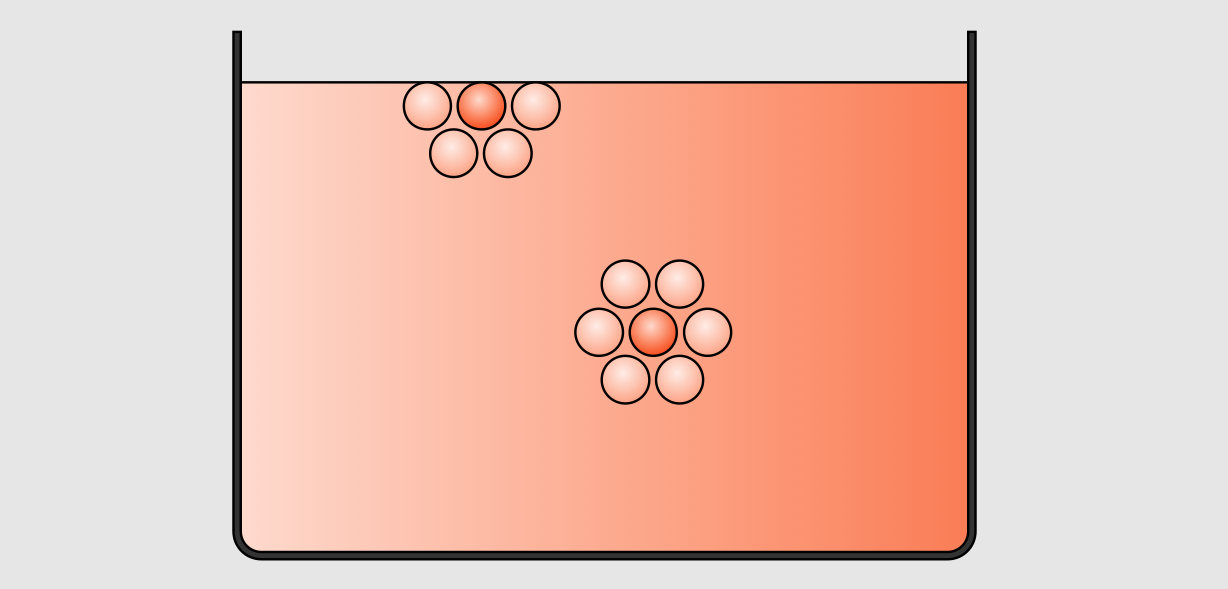
\includegraphics[width=0.5\linewidth]{Oberflaechenspannung.png}
 \caption{Modell zur Oberflächenspannung aus \cite[S. 198]{gerthsen} }
\end{figure}
An der Oberfläche einer Flüssigkeit wirken also nur die Kräfte ins Innere der Flüssigkeit, während in der Flüssigkeit auf ein Molekül Kräfte von allen Seiten wirken und sich so ausgleichen.\\
Die Oberflächenspannung einer Flüssigkeit $\sigma$ ist durch den Energiegewinn $dW$ definiert, der sich ergibt wenn sie eine Oberfläche $dA$ benetzt: $ \sigma=\frac{dW}{dA}$\\
Ist eine Kapillare mit Radius $r$ und eine Flüssigkeit mit der Oberflächenspannung $\sigma$ und der Dichte $\rho$ gegeben, so wird diese in der Kapillare um $h$ ansteigen, da sie durch das Benetzen Energie gewinnt.
Diese wird in potentielle Energie umgewandelt.
Es gilt also:
$$ \sigma\cdot A=mgh$$
Dabei ist $A=2\pi~r \cdot h$ und $m=\rho \pi ~ r^2 \cdot h$.
Für die Steighöhe $h$ folgt also:
\begin{align}
	h = \frac{2\sigma}{\rho~g~r}
\end{align}
oder für die Oberflächenspannung $\sigma$
\begin{align}
 \sigma =\frac{1}{2}h~\rho~g~r \label{eq:oberfl}
\end{align}
Man unterscheidet zwischen \textit{Kohäsion}, Kräfte zwischen gleichartigen Molekülen, und \textit{Adhäsion}, Kräfte, die an Grenzschichten auftreten.\\


\subsubsection{Mohrsche Waage}
Mit der Mohrschen Waage kann man die Dichte einer Flüssigkeit bestimmen.
Sie beruht auf dem \textit{archimedische Prinzip}, welches besagt, dass die Auftriebskraft eines Körpers so groß ist, wie die Gewichtskraft der verdrängten Flüssigkeit.\\
\begin{figure}[!htb]
	\centering
	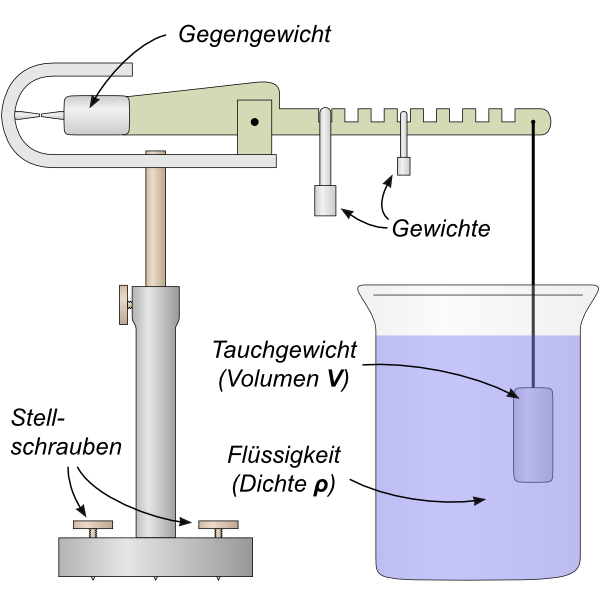
\includegraphics[scale=0.7]{MohrscheWaage.png}
	\caption{Mohrsche Waage \cite{lp}}
	\label{fig:MohrscheWaage}
\end{figure}
Zuerst wird die Waage außerhalb der Flüssigkeit so eingestellt, dass sie sich in der Gleichgewichtslage befindet.
Dann taucht man den Probekörper in die Flüssigkeit, deren Dichte bestimmt werden soll.
Aufgrund der Auftriebskraft beginnt der Körper zu steigen.
Deshalb hängt man an die Hebelarmseite des Probekörpers kleine Gewichte verschiedener Massen und in unterschiedlichem Abstand zum Drehpunkt, sodass die Gleichgewichtslage wiederhergestellt wird.
Das von diesen Gewichten verursachte Drehmoment entspricht dem Drehmoment der Auftriebskraft.
Wenn man das Volumen des Probekörpers nicht kennt, muss zuerst Wasser als Referenz genommen werden.\\
\begin{align}
\rho_F=\frac{\sum\limits_{i=1}^nm_{F,i}\cdot r_{F,i}}{\sum\limits_{i=1}^nm_{W,i}\cdot r_{W,i}}\cdot\rho_W
\end{align}
Dabei ist $m_{F,i}$ die i-te Masse der Flüssigkeit F, welche im Abstand $r_{F,i}$ angehängt wurde.
$\rho_W$ bezeichnet hierbei die Dichte von Wasser, die   $\rho_W\approx 997~\si{\kilo\gram/\meter^3}$ beträgt \cite[S. 258]{gerthsen}.
\subsection{Viskosität}
Viskosität ist ein Maß dafür, wie zähflüssig eine Flüssigkeit ist, also wie stark die innere Reibung ist.\\
Man unterscheidet zwei Fälle von Strömungen, wenn ein Körper von einem anderen Medium  umflossen wird:
\begin{itemize}
	\item \textit{laminare} Strömung: Das Fluid strömt in Schichten, die sich nicht miteinander vermischen. %wikipedia
	\item \textit{turbulente} Strömung: Es kommt zu Verwirbelungen. Die Beschreibung dieser ist sehr komplex, soll hier aber nicht näher betrachtet werden.
\begin{figure}[htb]
  \centering
  \subfigure[Laminare Strömung\label{fig:laminar}]
  {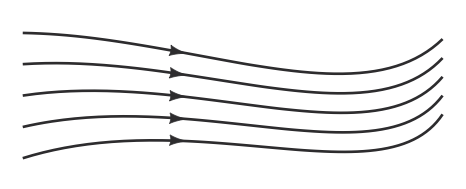
\includegraphics[width=0.50\textwidth]{laminar}}
  \hfill
  \subfigure[Turbulente Strömung\label{fig:turbulent}]
  {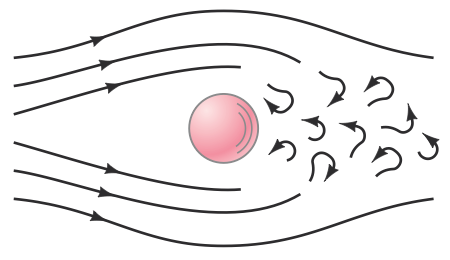
\includegraphics[width=0.45\textwidth]{turbulent}}
  \caption{Verschiedene Strömungsarten aus \cite[S. 465]{giancoli}}
  \label{fig:label-gesamt}
\end{figure}
\end{itemize}
Die Reynoldszahl $Re$ ist ein Maß für den Übergang von laminarer zu turbulenter Strömung.
Sie ist so definiert:
\begin{align}
	Re=\frac{\rho~v~d}{\eta}
\end{align}
mit der Dichte $\rho$, der Fließgeschwindigkeit $v$, der charakteristischen Länge $d$ des umflossenen Gegenstandes und der Viskosität $\eta$ der Flüssigkeit.\\
Diese wird durch die folgende Bewegungsgleichung von Flüssigkeiten unter innerer Reibung definiert:
\begin{align}
	F=\eta~ A\frac{dv}{dr}
\end{align}
Setzt man diese Kraft gleich der Druckkraft $F_p=\pi r^2 \cdot (p_1-p_2)$ kann das \textit{Hagen-Poiseuille Gesetz} der laminaren Rohrströmung hergeleitet werden, welches den Volumenstrom $\dot V$ durch ein Rohr der Länge $l$ und des Radiuses $r$ beschreibt.\cite[S.125]{gerthsen} % hier muss noch ergänzt werden
\begin{align}
	\dot{V}=\frac{\pi(p_1-p_2)}{8\eta l}r^4\label{eq:eta1}
\end{align}

\section{Durchführung}
\label{sec:durchfuehrung}
Zuerst werden die Durchmesser der 3 verschiedenen Kapillaren jeweils dreimal mit dem Messmikroskop vermessen.
Dabei wird die Kapillare fokussiert, dann der linke oder rechte Rand anvisiert.
Die Stellung der Micrometerschraube wird abgelesen, bevor man die gegenüberliegende Seite anvisiert und erneut die Skala abliest.
Aus der Differenz der beiden ergibt sich der Durchmesser der Kapillare.\\
Bei den Versuchen wird Methanol verwendet, welches giftig ist.
Auch Ethylenglykol ist gesundheitsschädlich.
Deshalb ist bei allen Versuchen der Kontakt mit diesen zu vermeiden.

\subsection{Kapillarität}
Man reinigt die Kapillaren gründlich mit Lösungsmittel und destilliertem Wasser, bevor man sie mit der Wasserstrahlpumpe trocknet.
Dieser Vorgang muss später nach jeder Flüssigkeit wiederholt werden.
Dabei ist darauf zu achten, dass beim Trocknen alle Flüssigkeitsreste entfernt werden und sich ganz besonders kein Film am oberen Ende bildet, der einen erheblich größeren Wiederstand beim Steigen hervorrufen würde.\\
Nun füllt man sich die drei auf Oberflächenspannung zu untersuchende Flüssigkeiten destilliertes Wasser, Methanol und Ethylenglykol in einen Becher ab.
Mithilfe der Mohr'schen Waage (Abb. \ref{fig:MohrscheWaage}) bestimmt man die jeweilige Dichte.
Dabei ist darauf zu achten, dass der Probekörper sauber ist und ganz in die Flüssigkeit eintaucht.\\
Dann misst man für jede der drei Flüssigkeiten und für jede der drei Kapillaren jeweils dreimal den Höhenunterschied $h_{Kap}$ der Flüssigkeitspegel, der sich ergibt, wenn man die Kapillare in die Flüssigkeit taucht und anschließend bis zur Oberfläche herauszieht.\\
Anschließend werden Methanol und Ethylenglykol in spezielle Behälter gegossen und somit vorschriftsmäßig entsorgt.
Nun müssen alle Gefäße und die Kapillaren gereinigt werden.
\begin{figure}[!htb]
	\centering
	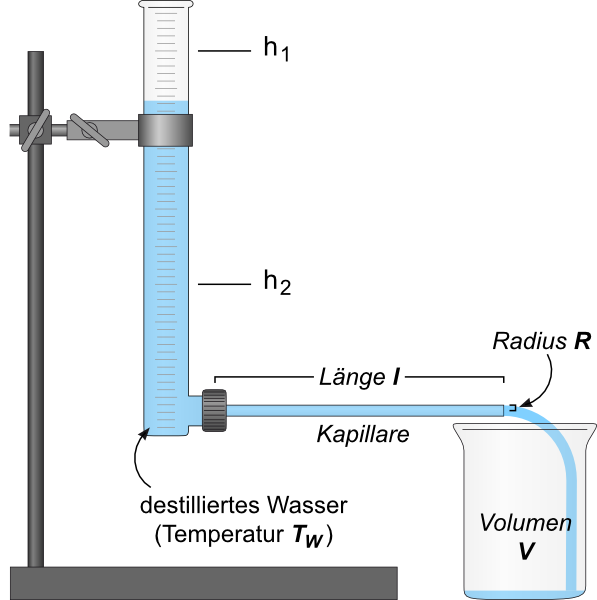
\includegraphics[scale=0.6]{ViskoAufbau.png}
	\caption{Versuchsaufbau zur Messung der Viskosität \cite{lp}}
	\label{fig:Visko}
\end{figure}
\subsection{Innere Reibung}
Zuerst misst man den Durchmesser des Glaszylinders und den Abstand der Strichmarken 50 und 45 von diesem, die Länge der Kapillaren und die Temperatur des destillierten Wassers.
Dann befestigt man eine der Kapillaren am Auslaufstutzen des Zylinders, hält die Öffnung zu und befüllt alles mit destillierten Wasser bis zur Strichmarke 50.
Es wird die Ausflusszeit bis zum Erreichen der Strichmarke 45 gemessen.
Dabei ist das ausfließende Wasser in einem Gefäß aufzufangen und wiederzuverwenden.
Diesen Vorgang wiederholt man auch für die anderen beiden Kapillaren.\\
Nun wählt man die Kapillare mit dem kleinsten Durchmesser und misst zu dieser während des Ausflusses die Zeit in Abhängigkeit der Höhe der Wassersäule.\\
Abschließend muss alles gesäubert werden und die Arbeitsfläche trocken gewischt werden.

\section{Auswertung}
\label{sec:auswertung}
\subsection{Dichte der drei Flüssigkeiten}
\begin{table}[!h]
\centering
\begin{tabular}{|l|c|c|c|}
\hline
 & Blau & Grün & Braun\\\hline
Durchmesser [mm]&$1.223\pm 0.014$&$1.811\pm 0.011$&$0.876\pm 0.018$\\\hline
Länge [cm]&$25.7\pm 0.1$&$ 25.5\pm 0.1$&$0.26\pm 0.1$\\\hline
\end{tabular}
\caption{Abmessungen der drei Kapillaren}
\end{table}
Um die Dichte von Methylalkohol und Ethylenglykol zu bestimmen, wurde die Mohr'sche Waage verwendet.
\begin{table}
\centering
\begin{tabular}{|c|c|c|c|c|}
\hline Aufhängung einzelner Gewichte & 5000mg & 500mg & 50mg &Dichte [kg/m$^3$]\\
\hline Dest. Wasser  & 10	&	& 1	& 997	\\
\hline Äthylenglykol & 10	& 9	& 3	& 1088	\\
\hline Methylalkohol & 8	& 4	& 	& 837	\\\hline
\end{tabular}
\caption{Position der einzelnen Gewichte an der Moor'schen Waage in Skalenteilen bei den unterschiedlichen Flüssigkeiten\label{tab:dichte}}
\end{table}
Die Literaturwerte nach \cite[S. 130-131]{Formelsammlung} lauten für Ethylenglykol 1113kg/m$^3$ (3\% größer, als unsere Messung) und für Methanol 790kg/m$^3$ (6\% kleiner, als unsere Messung).
\subsection{Oberflächenspannung}
Die Fehler der Oberflächenspannung nach Formel \eqref{eq:oberfl} berechnen sich nach
\begin{align*}
\sigma_{\sigma}=\frac{g}{2} \cdot \sqrt{h^{2} \cdot r^{2} \cdot \sigma_{\rho}^{2} + h^{2} \cdot \rho^{2} \cdot \sigma_{r}^{2} + r^{2} \cdot \rho^{2} \cdot \sigma_{h}^{2}}
\end{align*}
\begin{table}[!h]
\centering
\begin{tabular}{|l|l|c|c|}
\hline
Flüssigkeit 	     &Kapillar 	& m. Steighöhe [cm]		& Oberflächenspannung [N/m]\\\hline\hline
				&grün	& $1.45\pm 0.04$	&$ 0.0642 \pm 0.0017 $\\
Destiliertes Wasser		&blau	& $2.327\pm 0.035$	&$ 0.0696 \pm 0.0013 $\\
            			&braun	& $3.23\pm 0.04$	&$ 0.0693 \pm 0.0017 $\\\hline
				&grün	& $0.85\pm 0.04$	&$ 0.0411 \pm 0.0019 $\\
Ethylenglykol			&blau	& $1.383\pm 0.022$	&$ 0.0451 \pm 0.0009 $\\
				&braun	& $1.98\pm 0.06$	&$ 0.0464 \pm 0.0017 $\\\hline
				&grün	& $0.517\pm 0.022$	&$ 0.0192 \pm 0.0008 $\\
Methylalkohol			&blau	& $0.98\pm 0.10$	&$ 0.0247 \pm 0.0024 $\\
				&braun	& $1.33\pm 0.04$	&$ 0.0240 \pm 0.0009 $\\
\hline
\end{tabular}
\caption{Steighöhe unterschiedlicher Flüssigkeiten in unterschiedlichen Kapillaren und die sich daraus ergebende Oberflächenspannung}
\end{table}
Damit kann man mithilfe des gewichteten Mittelwertes die Werte aus Tab. \ref{tab:sigma} errechnen.\\
\begin{table}[!h]
\centering
\begin{tabular}{|c||c|c|c|}
\hline
$\sigma$ 		& Gew. Mittelwert [\si{\newton/\meter}]	& Literaturwert [\si{\newton/\meter}]	& Abweichung\\\hline\hline
dest. Wasser 		& $ 0.0681 \pm 0.0009 $			&$0.07275$				&7\%	\\\hline 
Ethylenglykol 		& $ 0.0448 \pm 0.0007 $			&$0.0484$				&8\%	\\\hline 
Methanol		& $ 0.0215 \pm 0.0006 $			&$0.0226$				&5\%	\\ 
\hline 
\end{tabular} 
\caption{Oberflächenspannung der drei Flüssigkeiten und deren Literaturwert nach \protect\footnotemark\label{tab:sigma}}
\end{table}
\footnotetext{http://de.wikipedia.org/wiki/Oberflächenspannung\#Werte}
\subsection{Viskosität}
\subsubsection{Viskosität aus Fließzeit}
Da uns aus zeitlichen Gründen leider die Messung der mittleren (blauen) Kapillaren unmöglich war, konnten wir nur die Viskosität der großen und der kleinen bestimmen.
Diese haben wir nach der Formel
\begin{align}
	\eta=\frac{\pi \cdot \Delta p \cdot dt \cdot r^{4}}{8 dV~ l}
\end{align}
berechnet und deren Fehler ergaben sich durch
\begin{align}
 \sigma_{\eta}=\frac{\pi r^{3}}{8  dV^{2} l^{2}} \sqrt{ dV^{2} l^{2} \left(16 \Delta p^{2} dt^{2} \sigma_{r}^{2} + \Delta p^{2} r^{2} \sigma_{dt}^{2} + dt^{2} r^{2} \sigma_{\Delta p}^{2}\right) +\Delta p^{2}r^{2}dt^{2} \left(dV^{2}   \sigma_{l}^{2} + l^{2} \sigma_{dV}^{2}\right)}\label{eq:sigmaeta}
\end{align}
wodurch wir für die beidem Messreihen die Ergebnisse der Tabelle \ref{tbl:viskozeit} erhielten
\begin{table}[!h]
 \centering
 \begin{tabular}{|c|c|c|}
  \hline
  Kapillar & Zeit [s] & Viskosität [Pa s]\\\hline
  grün & $5.54\pm 0.5$ & $0.0011\pm 0.0001$\\
  braun & $65.26\pm 0.5$&$0.00069\pm 0.00008$\\\hline
  gew. Mittelwert & & $0.00085\pm 0.00007$\\\hline
 \end{tabular}
 \caption{Bestimmung der Viskosität von Wasser bei verschiedenen Kapillaren aus deren jeweiligen Ausflusszeiten für von Markierung 50 bis 45\label{tbl:viskozeit}}
\end{table}

\subsubsection{Viskosität aus Fließgeschwindigkeit}
\begin{figure}
\centering
% GNUPLOT: LaTeX picture with Postscript
\begingroup
  \makeatletter
  \providecommand\color[2][]{%
    \GenericError{(gnuplot) \space\space\space\@spaces}{%
      Package color not loaded in conjunction with
      terminal option `colourtext'%
    }{See the gnuplot documentation for explanation.%
    }{Either use 'blacktext' in gnuplot or load the package
      color.sty in LaTeX.}%
    \renewcommand\color[2][]{}%
  }%
  \providecommand\includegraphics[2][]{%
    \GenericError{(gnuplot) \space\space\space\@spaces}{%
      Package graphicx or graphics not loaded%
    }{See the gnuplot documentation for explanation.%
    }{The gnuplot epslatex terminal needs graphicx.sty or graphics.sty.}%
    \renewcommand\includegraphics[2][]{}%
  }%
  \providecommand\rotatebox[2]{#2}%
  \@ifundefined{ifGPcolor}{%
    \newif\ifGPcolor
    \GPcolortrue
  }{}%
  \@ifundefined{ifGPblacktext}{%
    \newif\ifGPblacktext
    \GPblacktexttrue
  }{}%
  % define a \g@addto@macro without @ in the name:
  \let\gplgaddtomacro\g@addto@macro
  % define empty templates for all commands taking text:
  \gdef\gplbacktext{}%
  \gdef\gplfronttext{}%
  \makeatother
  \ifGPblacktext
    % no textcolor at all
    \def\colorrgb#1{}%
    \def\colorgray#1{}%
  \else
    % gray or color?
    \ifGPcolor
      \def\colorrgb#1{\color[rgb]{#1}}%
      \def\colorgray#1{\color[gray]{#1}}%
      \expandafter\def\csname LTw\endcsname{\color{white}}%
      \expandafter\def\csname LTb\endcsname{\color{black}}%
      \expandafter\def\csname LTa\endcsname{\color{black}}%
      \expandafter\def\csname LT0\endcsname{\color[rgb]{1,0,0}}%
      \expandafter\def\csname LT1\endcsname{\color[rgb]{0,1,0}}%
      \expandafter\def\csname LT2\endcsname{\color[rgb]{0,0,1}}%
      \expandafter\def\csname LT3\endcsname{\color[rgb]{1,0,1}}%
      \expandafter\def\csname LT4\endcsname{\color[rgb]{0,1,1}}%
      \expandafter\def\csname LT5\endcsname{\color[rgb]{1,1,0}}%
      \expandafter\def\csname LT6\endcsname{\color[rgb]{0,0,0}}%
      \expandafter\def\csname LT7\endcsname{\color[rgb]{1,0.3,0}}%
      \expandafter\def\csname LT8\endcsname{\color[rgb]{0.5,0.5,0.5}}%
    \else
      % gray
      \def\colorrgb#1{\color{black}}%
      \def\colorgray#1{\color[gray]{#1}}%
      \expandafter\def\csname LTw\endcsname{\color{white}}%
      \expandafter\def\csname LTb\endcsname{\color{black}}%
      \expandafter\def\csname LTa\endcsname{\color{black}}%
      \expandafter\def\csname LT0\endcsname{\color{black}}%
      \expandafter\def\csname LT1\endcsname{\color{black}}%
      \expandafter\def\csname LT2\endcsname{\color{black}}%
      \expandafter\def\csname LT3\endcsname{\color{black}}%
      \expandafter\def\csname LT4\endcsname{\color{black}}%
      \expandafter\def\csname LT5\endcsname{\color{black}}%
      \expandafter\def\csname LT6\endcsname{\color{black}}%
      \expandafter\def\csname LT7\endcsname{\color{black}}%
      \expandafter\def\csname LT8\endcsname{\color{black}}%
    \fi
  \fi
  \setlength{\unitlength}{0.0500bp}%
  \begin{picture}(7200.00,5040.00)%
    \gplgaddtomacro\gplbacktext{%
      \csname LTb\endcsname%
      \put(1078,704){\makebox(0,0)[r]{\strut{} 3.65}}%
      \put(1078,1382){\makebox(0,0)[r]{\strut{} 3.7}}%
      \put(1078,2061){\makebox(0,0)[r]{\strut{} 3.75}}%
      \put(1078,2739){\makebox(0,0)[r]{\strut{} 3.8}}%
      \put(1078,3418){\makebox(0,0)[r]{\strut{} 3.85}}%
      \put(1078,4096){\makebox(0,0)[r]{\strut{} 3.9}}%
      \put(1078,4775){\makebox(0,0)[r]{\strut{} 3.95}}%
      \put(1210,484){\makebox(0,0){\strut{} 0}}%
      \put(2009,484){\makebox(0,0){\strut{} 20}}%
      \put(2808,484){\makebox(0,0){\strut{} 40}}%
      \put(3607,484){\makebox(0,0){\strut{} 60}}%
      \put(4406,484){\makebox(0,0){\strut{} 80}}%
      \put(5205,484){\makebox(0,0){\strut{} 100}}%
      \put(6004,484){\makebox(0,0){\strut{} 120}}%
      \put(6803,484){\makebox(0,0){\strut{} 140}}%
      \put(176,2739){\rotatebox{-270}{\makebox(0,0){\strut{}logarithmische Höhe [ln(Skalenteile)]}}}%
      \put(4006,154){\makebox(0,0){\strut{}Zeit [s]}}%
    }%
    \gplgaddtomacro\gplfronttext{%
      \csname LTb\endcsname%
      \put(2662,4602){\makebox(0,0)[r]{\strut{}Messpunkte}}%
      \csname LTb\endcsname%
      \put(2662,4382){\makebox(0,0)[r]{\strut{}Fit}}%
    }%
    \gplbacktext
    \put(0,0){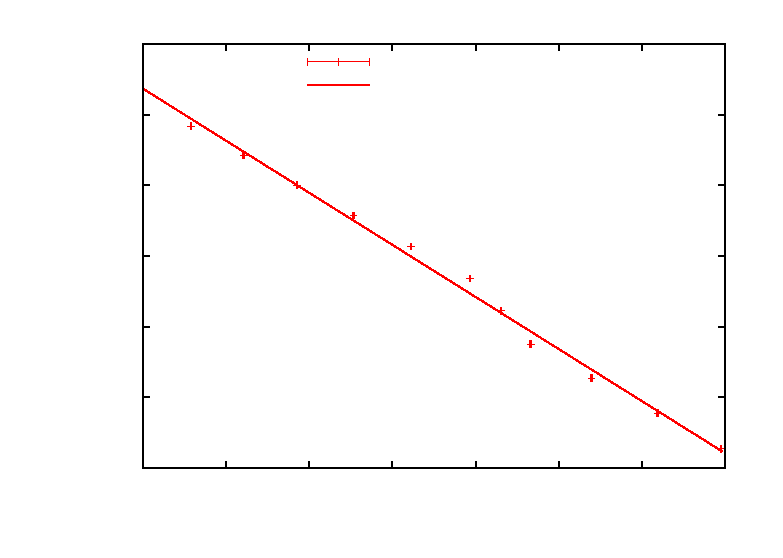
\includegraphics{Viskositaet}}%
    \gplfronttext
  \end{picture}%
\endgroup

\caption{Messung der Viskosität von Wasser halblogarithmisch aufgetragen\label{fig:viskogerade}}
\end{figure}
Die Fehlerfortpflanzung der Viskosität der umgestellten Formel \eqref{eq:eta1} in deren Diskretisierung ist analog zu Formel \eqref{eq:sigmaeta}, wodurch sich die Werte und deren Fehler aus Tabelle \ref{tbl:visko2b} ergeben.\\
Aus der Geradensteigung $m$ der gefitteten Daten aus Abb. \ref{fig:viskogerade} berechnet sich mit
\begin{align}
 \eta=-\frac{\rho g R^4}{8mlr^2}
\end{align}
ein Wert von $\eta=(0.00060 \pm 0.00007)\si{\Pa\s}$. Die Diskrepanz der beiden Werte der Geradensteigung und der Tabelle \ref{tbl:visko2b} ist dadurch zu erklären, dass bei dem Fit auch der Wert der Zeit $t=74.48$s mit berücksichtigt wurde, den wir aus Tablelle explizit herausgenommen haben (s. Diskussion). Andernfalls käme man auf ein identisches Ergebnis.\\
Der Literaturwert\footnote{Quelle: www.uni-magdeburg.de/isut/LSS/Lehre/Arbeitsheft/IV.pdf, Seite 1, 22.06.2014, 13 Uhr} der Viskosität von Wasser für $\SI{25}{\celsius}$ liegt bei 0.00089 \si{\Pa\s} was 25\% größer ist, als die Tabellenmesswerte, welche für $(27.5\pm 1)^\circ$C aufgenommen wurden. Allerdings ist nach eben dieser Quelle die Viskosität von Wasser bei $30^\circ$C nurnoch bei 0.000798 \si{\Pa\s}, was nurnoch 12\% größer ist, als unser Wert.
\begin{table}[!h]
\centering
\begin{tabular}{|l|l|}
 \hline
Zeitunterschied [s] & Viskosität [Pa s]\\
\hline\hline
\num{11.66} & $0.00063 \pm 0.00007$\\
\hline
\num{12.57} & $0.00068 \pm 0.00008$\\
\hline
\num{12.84} & $0.00068 \pm 0.00008$\\
\hline
\num{13.61} & $0.00072 \pm 0.00008$\\
\hline
\num{13.84} & $0.00072 \pm 0.00008$\\
\hline
\num{14.15} & $0.00073 \pm 0.00009$\\
\hline
\num{14.58} & $0.00074 \pm 0.00009$\\
\hline
\num{14.63} & $0.00074 \pm 0.00009$\\
\hline
\num{15.78} & $0.00079 \pm 0.00009$\\
\hline
\num{15.33} & $0.00076 \pm 0.00009$\\
\hline\hline
gew. Mittelwert & $0.00071 \pm 0.00003$\\
\hline
\end{tabular}
\caption{Versuch 2b - Messung der Viskosität von Wasser in unterschiedlichen Zeitdifferenzen und deren resultierende Viskosität zusammen mit dem gewichteten Mittelwert\label{tbl:visko2b}}
\end{table}
\section{Diskussion}
\label{sec:diskussion}
Bei der Bestimmung der Dichte mit der Mohr'schen Waage stellten wir fest, dass die Eichung der Waage sich augenscheinlich während der Messung leicht verstellte.
So haben wir bei den drei Messungen jeweils eine Abweichung nach der Messung von der Gleichgewichtslage gehabt.
Diese haben wir natürlich vor jeder Messung wiederhergestellt, allerdings können dadurch unsere Messergebnisse der Dichte natürlich verfälscht sein.\\
Aufgrund von fehlender Zeit schafften wir es leider nicht, die Messung der Ausflusszeit des mittleren Kapillars zu bestimmen.
Da wir jedoch die Messungen des kleinen und großen Kapillars durchführen konnten, haben wir wenigstens einen Eindruck bekommen, wie die Kapillardicke mit der Ausflussgeschwindigkeit zusammenhängt.\\
Bei dem zweiten Teilversuch der Viskosität haben wir offensichtlich einen falschen Messwert notiert.
Schon ein oberflächlicher Blick zeigt hier, dass für die Werte 52.86s, 67.01s, 74.48s, 81.59s und 96.22s die Differenz zum nächsten nicht annähernd ähnlich ist.
Ohne den Wert von 74.48s zu berücksichtigen, kamen wir auf konsistente Werte und wir schlossen diesen aus, da wir vermuten, einen zusätzlichen Wert für einen halben Skalenschritt hier aufgenommen zu haben.\\
Bei der Suche der Literaturwerte hatten wir teilweise Probleme, geeignete Werte zu finden, da es nur wenige (und zudem nicht besonders vertrauenswürdige) Quellen zur Viskosität gibt, welche zudem höchstens die jeweiligen Werte zu 25\si{\celsius} hatten, was nicht unseren gemessenen $(27.5\pm 1)$\si{\celsius} übereinstimmt.\\\\
Insgesamt erhielten wir bei allen Messungen gute Werte mit Abweichungen von den Literaturwerten von um die 10\%.
Dies ließ sich nur realisieren, da bei der Reinigung der Kapillaren besonders darauf geachtet wurde, Rückstände der Reinigungsmittel möglichst komplett zu entfernen und vor allem Flüssigkeitsblasen in den Kapillaren zu vermeiden, die einen starken Einfluss auf die Messergebnisse (insbesondere der Kapillarität) hätten.


\section{Anhang}
\begin{thebibliography}{9}

\bibitem{lp} 
	\emph{Lehrportal der Universität Göttingen, Kapillarität und Viskosität},
  https://lp.uni-goettingen.de/get/text/3638, abgerufen 22.06.14 18:32 Uhr

\bibitem{gerthsen}
	\textsc{Dieter Meschede} (2010): \emph{Gerthsen Physik}, 24. Auflage, Springer Heidelberg
Dordrecht London New York

\bibitem{Formelsammlung}
	\textsc{Wolfgang Pfeil et. al.} (2009): \emph{Das große Tafelwerk (interaktiv)}, 1. Auflage, Cornelsen Berlin

\bibitem{giancoli}
	\textsc{Douglas C. Giancoli} (2010): \emph{Physik - Lehr- und Übungsbuch}, 3. Auflage, Pearson Studium London
\end{thebibliography}


\end{document}
